\section{Particle composition and detector response of hadronic recoil}

This section examines the particle composition and the detector response of the leading jet that balance the $Z$~boson in the fiducial region of the analysis. 
The Powheg $Z\to \mu\mu$ sample is used. The particle origin of each track is obtained using the \texttt{truthParticleLink} to find the truth identification of each reconstructed track (see section~\ref{sec:samples}). In addition to the standard event preselection described in section~\ref{sec:selection}, extra cuts are used to make sure the leading reconstructed jet matches the leading particle jet in each event. 
%To ensure the closet matching between the leading reconstructed jet and leading truth jet, and always have very good DR between them, the cut on ratio of 
This is achieved by requiring $|y_\mathrm{j1}|<2.1$ and $\pTlj / \pTsj < 0.7$. The selection is applied on reconstructed level. However, due to the additional criterion, the leading particle-level (truth) jet will always match the leading reco jet. Note that the jets will have a very high \pt{} since the event selection includes the selection $\pTll > \SI{165}{\GeV}$, and the jet will have a similar \pt{} to that of the $Z$~boson.

Particles are classified depending to their type in the following categories: \texttt{pion} for $\pi^+$ and $\pi^-$; \texttt{kaon}; \texttt{proton}; 
\texttt{mu} for $\mu^-$ or $\mu^+$; \texttt{e} for $e^-$ or $e^+$;
strange for any charge hadron with strange content other than kaons; \texttt{neutral} for any neutral hadron; \texttt{gam} for photons. As mentioned above, tracks are classified in the same categories using the \texttt{truthParticleLink}. In case there is no truth particle match, it is labelled unmatched. This includes contributions from pileup particles and fake tracks (and possibly secondaries).


All of the reconstructed tracks inside leading jet as well as charged-particles in the associated particle-level jets that are not matched to reconstructed tracks are used for the plots shown in this section. Figure~\ref{fig:fraction of charged particles in reco jet} shows the fraction of the particle multiplicity (left) as a function of the truth jet \pT. The 78\% of reconstructed tracks make up pions about of the total, kaons are about 12\% of the total, protons are about 4\%, unmatched tracks are around 5\% and strange are almost 1\%. The momentum fraction as a function of jet pT is shown in right in Figure~\ref{fig:fraction of charged particles in reco jet}. The momentum fraction for different particles varies slightly as compare to multiplicity fraction.

\begin{figure}[b]
	\centering
	\includegraphics[width=0.48\textwidth,page=3]{figures/jet_comp_study_powheg_Tight_MultiplicityFraction.pdf}
	\includegraphics[width=0.48\textwidth,page=3]{figures/jet_comp_study_powheg_Tight_pTFraction.pdf}
	\caption{Composition of the leading jet in terms of particle multiplicity (left) and \pt{} (right) as a function of jet \pt{}.
		The photon multiplicity is divided by 2 in the left plot, since most photons are produced in pairs by a neutral hadron (e.g.\ $\pi\to\gamma\gamma$). 
		We can see that $\approx 42$\% of the jet \pt{} is carried by neutral particles. It's surprising that the fraction of neutral hadrons is so high (why??).}
	\label{fig:truthJetComp}
\end{figure}


\begin{figure}
\centering
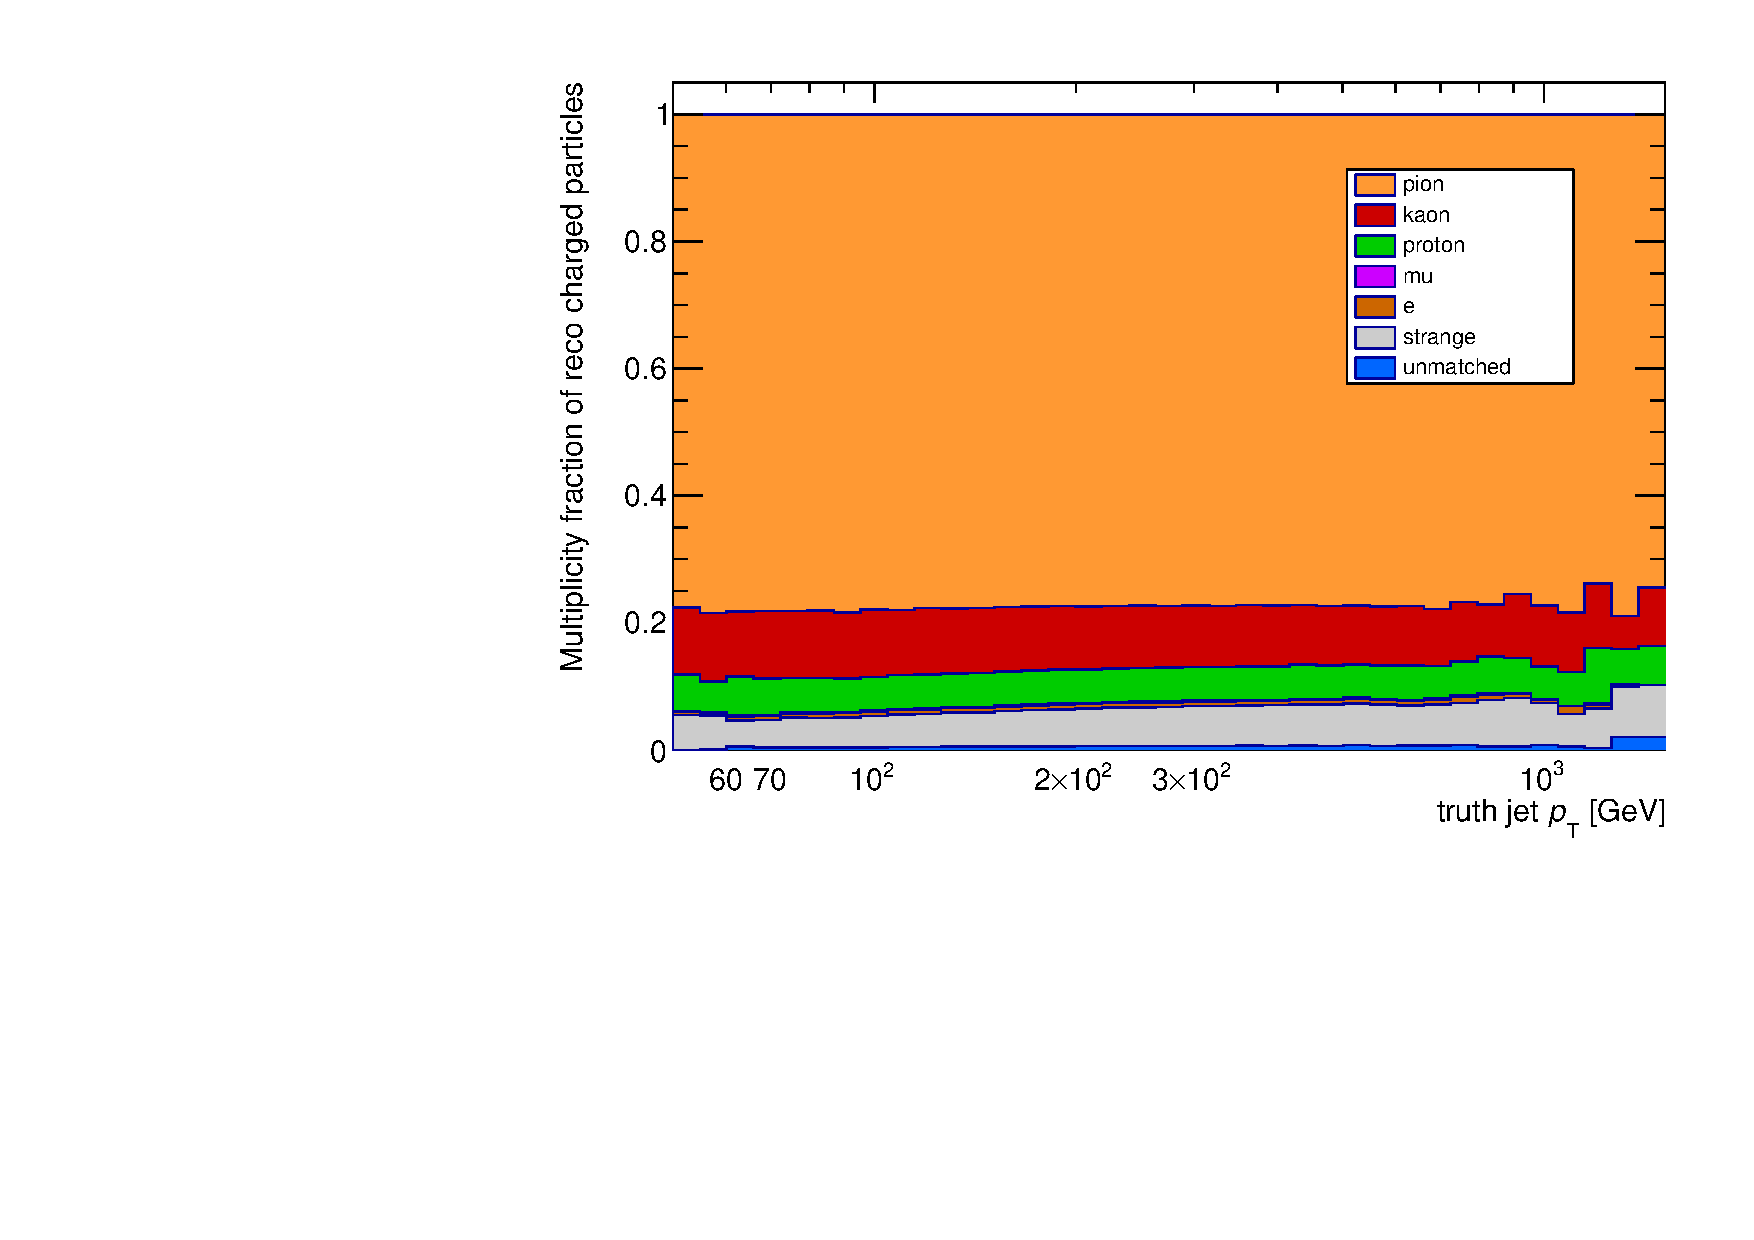
\includegraphics[width=0.48\textwidth,page=1]{figures/jet_comp_study_powheg_Tight_MultiplicityFraction.pdf}
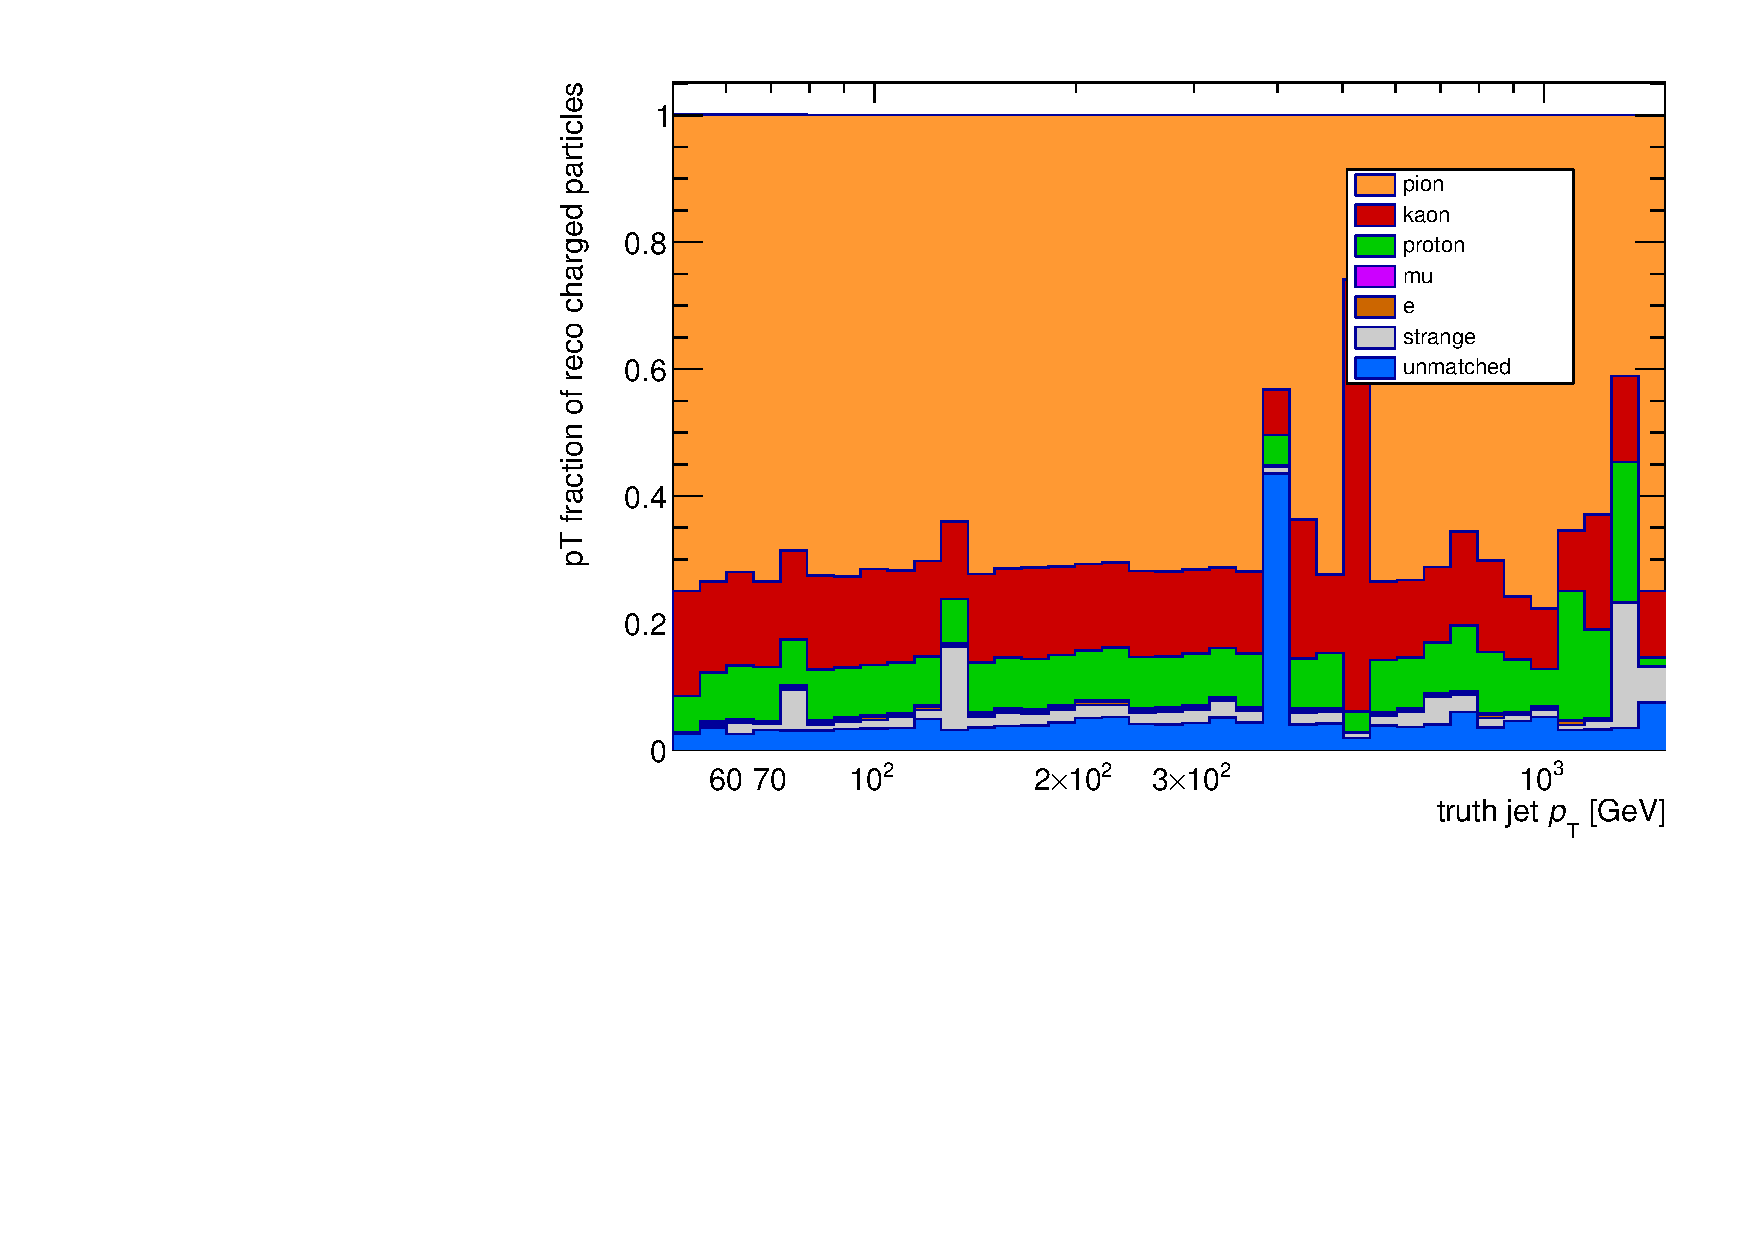
\includegraphics[width=0.48\textwidth,page=1]{figures/jet_comp_study_powheg_Tight_pTFraction.pdf}
\caption {The fraction of the reconstructed tracks multiplicity (left) and \pT (right) inside reconstructed leading jet as a function of jet pT for various categories (see the text for details).}
\label{fig:fraction of charged particles in reco jet}
\end{figure}


\begin{figure}
\centering
\includegraphics[scale=0.3, page=2]{figures/jet_comp_study_powheg_Tight_MultiplicityFraction.pdf}
\hspace{2mm}
\includegraphics[scale=0.3, page=2]{figures/jet_comp_study_powheg_Tight_pTFraction.pdf}
\caption {The fraction of the charged particle multiplicity (left) and \pT (right) inside particle level leading jet as a function of jet pT for various categories (see the text for details).}
\label{fig:fraction of charged particles in truth jet}
\end{figure}

Figure~\ref{fig:fraction of charged particles in truth jet} shows the fraction of the charged particle multiplicity (left) and their \pT  as a function of the truth jet \pT in the particle-level jet. From charged particle compositions, mostly are pions ~74\%, kaons are 14\% and rest 12\% comprise other charged particle.
Figure~\ref{fig:fraction of charged particles in truth jet} shows similar plots for particle level jet, but for all the particle compositions in the leading jet. From the multiplicity fraction plot (left), it can be seen that ~43\% are photons which are ~20\% greater than in \pt fraction (right) dur to decay of pions into photons.


Figures~\ref{fig:response pion and kaon} to ~\ref{fig:track jet response} are showing the detector response for each particle category. The pion and kaon respose are ~93\% and ~94\% respectively which indicates tracking efficiency is around 93\%. Figure~\ref{fig:unmatched tracks fraction} depicts fraction of unmatched track w.r.t reco level jet, which indicates ~2\% tracking inefficiency. Similarly, figures~\ref{fig:fraction pions and kaons} to ~\ref{fig:response electrons and starnge particles} are showing the fraction of individual particles at truth level and reconstructed level. As shown in figure~\ref{fig:fraction of charged particles in truth jet}, pions make most of jet fraction, and for muons, electrons and strange particles this fraction is much lower. the muon and electron responses are very low because these particles come from semileptonic decay of heavy hadrons, so we have a displaced vertex

\begin{figure}
\centering
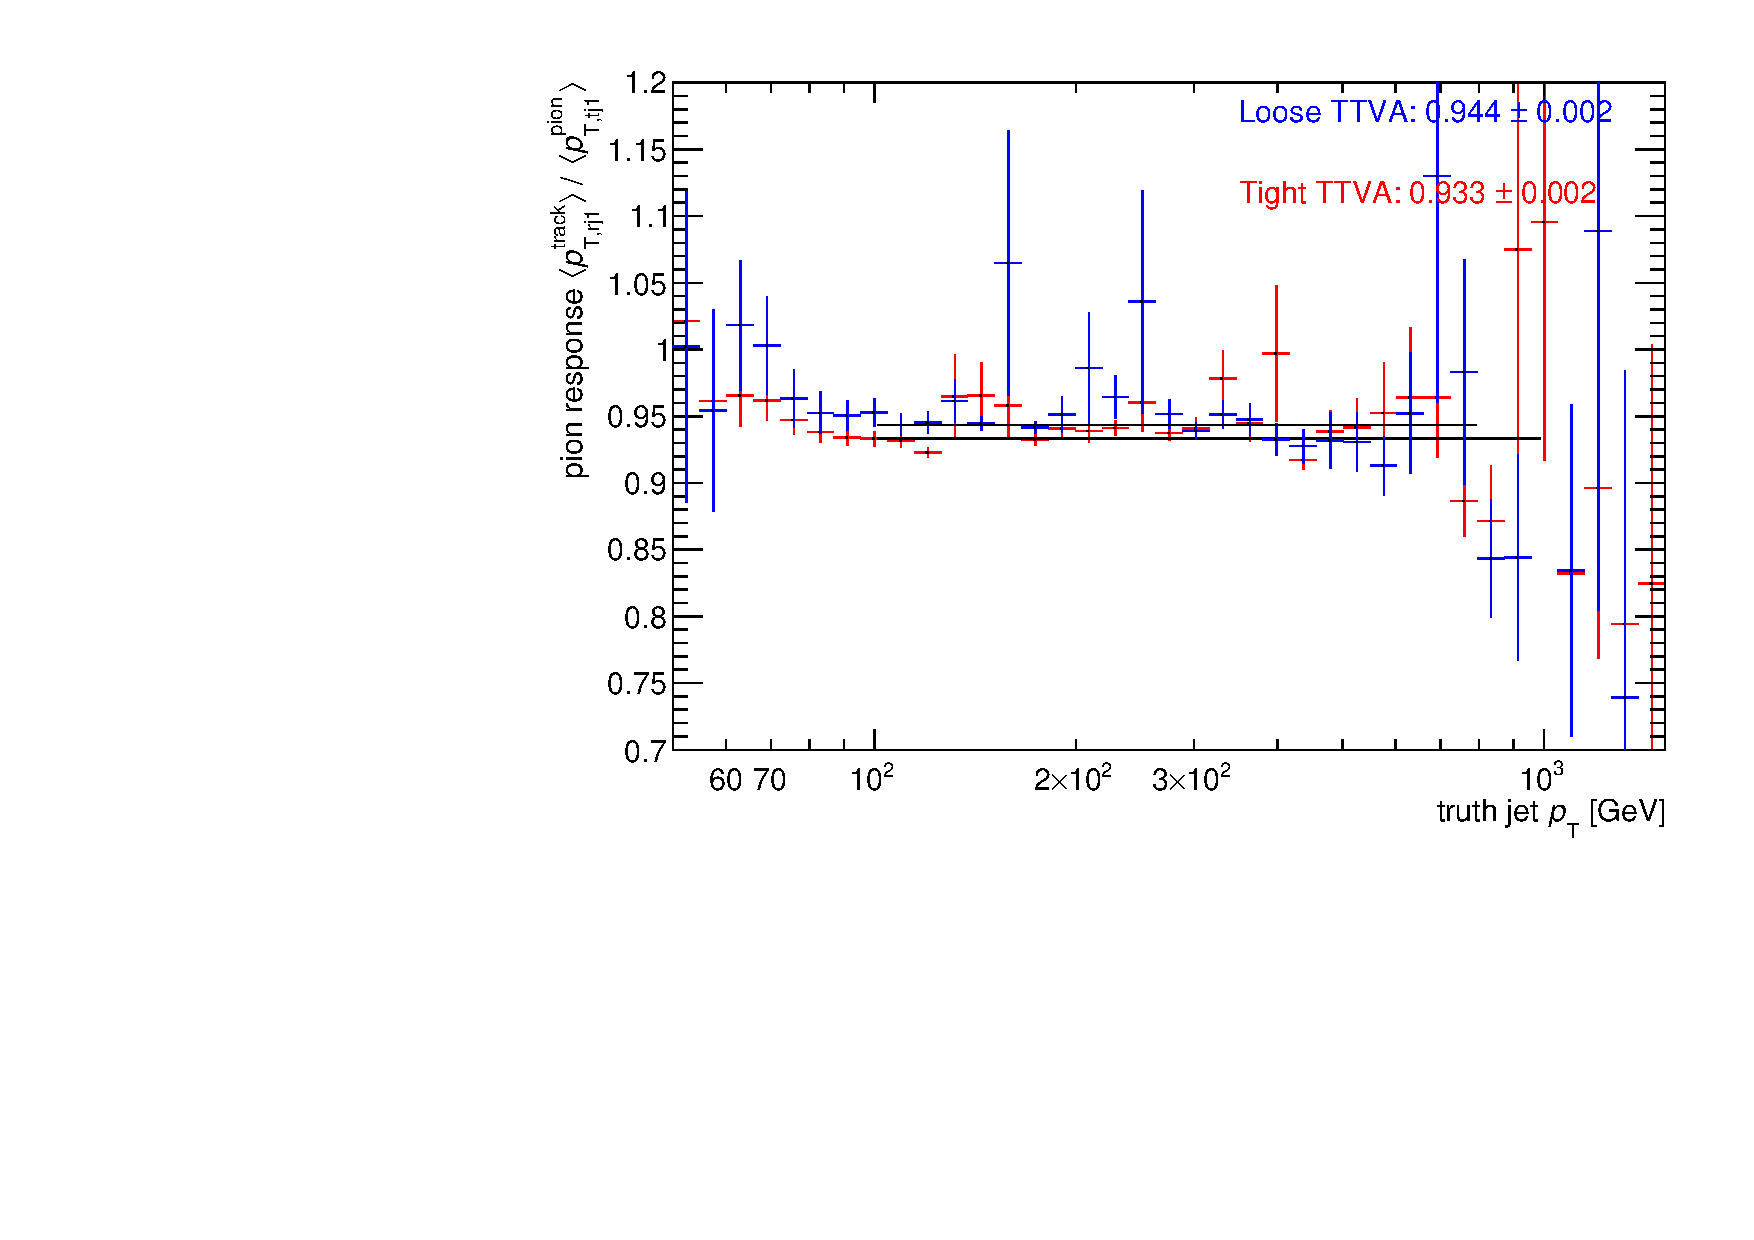
\includegraphics[scale=0.3, page=1]{figures/jet_comp_study_powheg_Tight_MultiplicityFraction_withLooseandTight.pdf}
\includegraphics[scale=0.3, page=2]{figures/jet_comp_study_powheg_Tight_MultiplicityFraction_withLooseandTight.pdf}
\caption {The response of pions (left) and  kaons (right) as a function of jet \pT.}
\label{fig:response pion and kaon}
\end{figure}

\begin{figure}
\centering
\includegraphics[scale=0.3, page=3]{figures/jet_comp_study_powheg_Tight_MultiplicityFraction_withLooseandTight.pdf}
\includegraphics[scale=0.3, page=4]{figures/jet_comp_study_powheg_Tight_MultiplicityFraction_withLooseandTight.pdf}
\caption {The response of protons (left) and  muons (right) as a function of jet \pT.}
\label{fig:response proton and muon}
\end{figure}

\begin{figure}
\centering
\includegraphics[scale=0.3, page=5]{figures/jet_comp_study_powheg_Tight_MultiplicityFraction_withLooseandTight.pdf}
\includegraphics[scale=0.3, page=6]{figures/jet_comp_study_powheg_Tight_MultiplicityFraction_withLooseandTight.pdf}
\caption {The response of electrons (left) and strange particles (right) as a function of jet \pT.}
\label{fig:response electron and starnge}
\end{figure}

\begin{figure}
\centering
\includegraphics[scale=0.3, page=7]{figures/jet_comp_study_powheg_Tight_MultiplicityFraction_withLooseandTight.pdf}
\caption {The response of  all the reconstructed tracks w.r.t charged particles as a function of jet \pT.}
\label{fig:track jet response}
\end{figure}

\begin{figure}
\centering
\includegraphics[scale=0.3, page=8]{figures/jet_comp_study_powheg_Tight_MultiplicityFraction_withLooseandTight.pdf}
\caption {The fraction of unmatched tracks w.r.t reco level jet as a function of jet \pT.}
\label{fig:unmatched tracks fraction}
\end{figure}


\begin{figure}
\centering
\includegraphics[scale=0.3, page=4]{figures/jet_comp_study_powheg_Tight_pTFraction.pdf}
\includegraphics[scale=0.3, page=5]{figures/jet_comp_study_powheg_Tight_pTFraction.pdf}
\caption {The fraction of pions (left) and kaons (right) in the reconstructed tracks as a function of jet \pT.}
\label{fig:fraction pions and kaons}
\end{figure}


\begin{figure}
\centering
\includegraphics[scale=0.3, page=6]{figures/jet_comp_study_powheg_Tight_pTFraction.pdf}
\includegraphics[scale=0.3, page=7]{figures/jet_comp_study_powheg_Tight_pTFraction.pdf}
\caption {The fraction of protons (left) and muons (right) in the reconstructed tracks as a function of jet \pT.}
\label{fig:response protons and muons}
\end{figure}


\begin{figure}
\centering
\includegraphics[scale=0.3, page=8]{figures/jet_comp_study_powheg_Tight_pTFraction.pdf}
\includegraphics[scale=0.3, page=9]{figures/jet_comp_study_powheg_Tight_pTFraction.pdf}
\caption {The fraction of electrons (left) and strange particles (right) in the reconstructed tracks as a function of jet \pT.}
\label{fig:response electrons and starnge particles}
\end{figure}